

% LaTeX file for Chapter 02


\chapter{Methods} 

In this section I will explain the necessary background needed to understand the TRAM-DAGs. Once the framework of tram dags is explained, I will present how the experiments of the simulation, the application on real data and the ITE estimation are conducted.


The goal of TRAM-DAGs is to estimate the structural equations according to the causal order in a given DAG in a flexible and possibly still interpretable way in order to sample observational and interventional distributions and to make counterfactual statements. The estimation requires data and a DAG that describes the causal structure. It must be assumed that there are no hidden confounders. TRAM-DAGs estimate for each variable $X_i$ a transformation function $Z_i = h_i(X_i \mid pa(X_i))$, where $Z_i$ is the noise value and $pa(X_i)$ are the causal parents of $X_i$. The important part here is that we can rearrange this equation to $X_i = h_i^{-1}(Z_i \mid pa(x_i))$ to get to the structural equation. The transformation functions $h$ are monotonically increasing functions that are a representation of the conditional distribution of $X_i$ on a latent scale. They are based on the idea of transformation models as introduced by \citet{hothorn2014} but were extended to deep trams by \citet{sick2020}. In the following sections I review the most important ideas of these methods as they are the essential components of TRAM-DAGs.

\section{Transformation Models}


Transformation models are a flexible distributional regression method for various data types. They can be for example specified as ordinary linear regression, logistic regression or proportional odds logistic regression. But Transformation models further allow to model conditional outcome distributions that do not even need to belong to a known distribution family of distributions by model it in parts flexibly. This reduces the strength of the assumptions that have to be made.

The basic form of transformation models can be described by

\begin{equation}
F(y|\mathbf{x}) = F_Z(h(y \mid \mathbf{x})) =  F_Z(h_I(y) - \mathbf{x}^\top \boldsymbol{\beta})
\label{eq:transformation_model}
\end{equation}

, where $F(y|\mathbf{x})$ is the conditional cumulative distribution function of the outcome variable $Y$ given the predictors $\mathbf{x}$. $h(y \mid \mathbf{x})$ is a transformation function that maps the outcome variable $y$ onto the latent scale of $Z$. $F_Z$ is the cumulative distribution function of a latent variable $Z$, the so-called inverse-link function that maps $h(y \mid \mathbf{x})$ to probabilities. In this basic version, the transformation function can be split into an intercept part $h_I(y)$ and a linear shift part $\mathbf{x}^\top \boldsymbol{\beta}$, where the vector $\mathbf{x}$ are the predictors and $\boldsymbol{\beta}$ are the corresponding coefficients.

If the latent distribution $Z$ is chosen to be the standard logistic distribution, then the coefficient $\beta_i$ can be interpreted as log-odds ratios when increasing the predictor $x_i$ by one unit, holding all other predictors unchanged. This means that an increase of one unit in the predictor $x_i$ leads to an increase of the log-odds of the outcome $Y$ by $\boldsymbol{\beta}$. The additive shift of the transformation function means a linear shift on the latent scale (herer log-odds). The following transformation to probabilities by $F_Z$ potentially leads to a non-linear change in the conditional outcome distribution on the original scale. This means not only is the distribution shifted, also its shape can change to some degree based on the covariates. More details about the choice of the latent distribution and the interpretation of the coefficients are provided in the appendix XXX.


For a continuous outcome $Y$ the intercept $h_I$ is represented by a bernstein polynomial, which is a flexible and monotonically increasing function

\begin{equation}
h_I(y) = \frac{1}{M + 1} \sum_{k=0}^{M} \vartheta_k \, \text{B}_{k, M}(y)
\end{equation}

, where $\vartheta_k$ are the coefficients of the bernstein polynomial and $\text{B}_{k, M}(y)$ are the Bernstein basis polynomials. More details about the technical implementation of the bernstein polynomial in the context of TRAM-DAGs is given in the appendix XXX.

For a discrete outcome $Y$ the intercept $h_I$ is represented by cut-points, which are the thresholds that separate the different levels of the outcome. For example, for a binary outcome $Y$ there is one cut-point and for an ordinal outcome with $K$ levels there are $K-1$ cut-points. The transformation model is given by

\begin{equation}
P(Y \leq y_k \mid \mathbf{X} = \mathbf{x}) = F_Z(\vartheta_k + \mathbf{x}^\top \boldsymbol{\beta}), \quad k = 1, 2, \ldots, K - 1
\end{equation}


A visual representation for a continuous and discrete (ordinal) outcome is provided in Figure~\ref{fig:tram_cont_ord}.


% include image /img/tram_cont_ord.png
\begin{figure}[H]
\centering
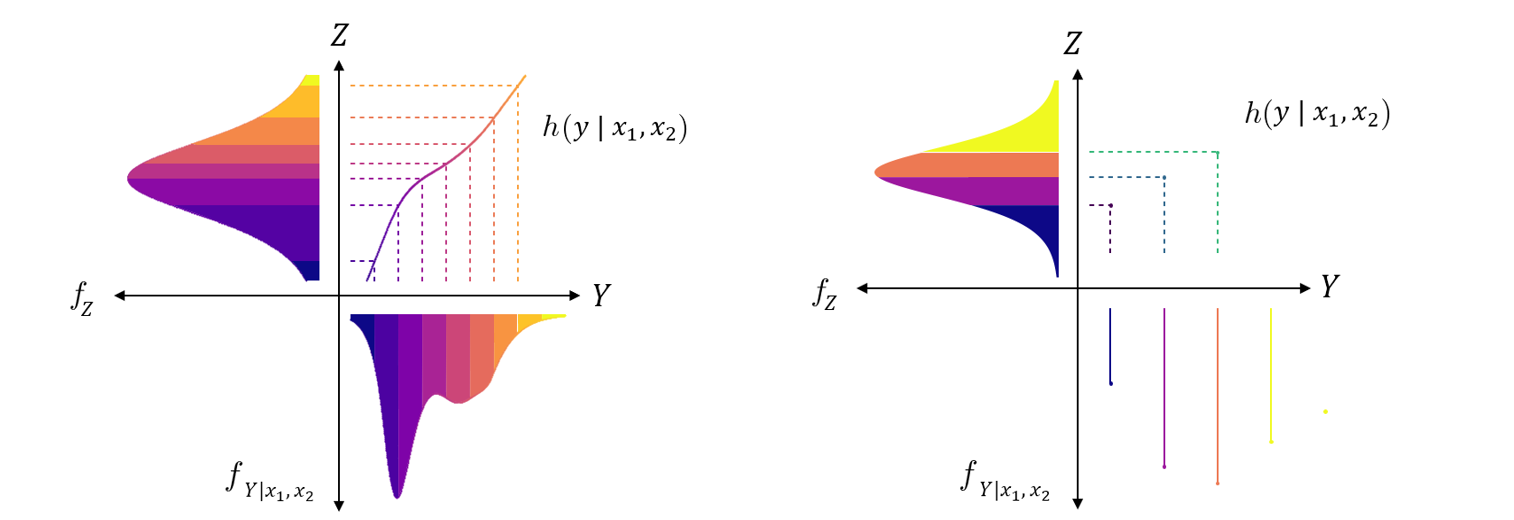
\includegraphics[width=1\textwidth]{img/tram_cont_ord.png}
\caption{\textbf{Left:} Example of a transformation model for a continuous outcome $Y$ with a smooth transformation function. \textbf{Right:} Example of a transformation model for an ordinal outcome $Y$ with 5 levels. The transformation function consists of cut-points that separate the probabilities for the levels of the outcome.
In both cases the latent distribution $Z$ is the standard logistic and the predictors $\mathbf{x}$ induce a linear (vertical) shift of the transformation function.}
\label{fig:tram_cont_ord}
\end{figure}


To estimate the parameters $\boldsymbol{\beta}$ and $\boldsymbol{\vartheta}$ the negative log likelihood (NLL) is minimized. The NLL is defined as

\begin{equation}
\text{NLL} = - \frac{1}{n} \sum_{i=1}^{n} l_i(\boldsymbol{\beta}, \boldsymbol{\vartheta} ) = - \frac{1}{n} \sum_{i=1}^{n} \log (f_{Y \mid \mathbf{X} = \mathbf{x}}(y_i))
\label{eq:nll_tram}
\end{equation}

where $l_i(\boldsymbol{\beta}, \boldsymbol{\vartheta})$ is the log-likelihood of the $i$-th observation,  $l_i(\boldsymbol{\beta}, \boldsymbol{\vartheta}) = f_{Y \mid \mathbf{X} = \mathbf{x}}(y_i)$ is the conditional density function of the outcome variable $Y$ given the predictors $\mathbf{x}$ under the current parameterization. I provide the full derivation in the appendix xxx.


For the remainder of this thesis, I rely on the idea of these transformation models to model the conditional distribution functions represented by the transformation functions of the respective variables. The standard logistic distribution is used as $F_Z$, which results in a logistic transformation model.


\section{Deep TRAMs} \label{sec:deep_trams}

The transformation models as discussed before were extended to deep TRAMs using a modular neural network \citep{sick2020}. The goal is to get a parametrized transformation function of the form \ref{eq:deep_tram.}.Each part, the intercept $h_I(X_i)$, the linear shift $\mathbf{x}_L^\top \boldsymbol{\beta}_L$ and the complex shift $f_C(\mathbf{x}_C)$ are assembled by the outputs of the individual neural networks. The user can specify the level of complexity the parents $pa(X_i)$ have on the transformaiton funciton. Figure \ref{fig:deep_tram} illustrates the case for a SI-LS-CS model.

\begin{equation}
h(y \mid \mathbf{x}_L, \mathbf{x}_C ) = h_I(y) + \mathbf{x}_L^\top \boldsymbol{\beta}_L + f_C(\mathbf{x}_C)
\label{eq:deep_tram}
\end{equation}



\begin{figure}[H]
\centering
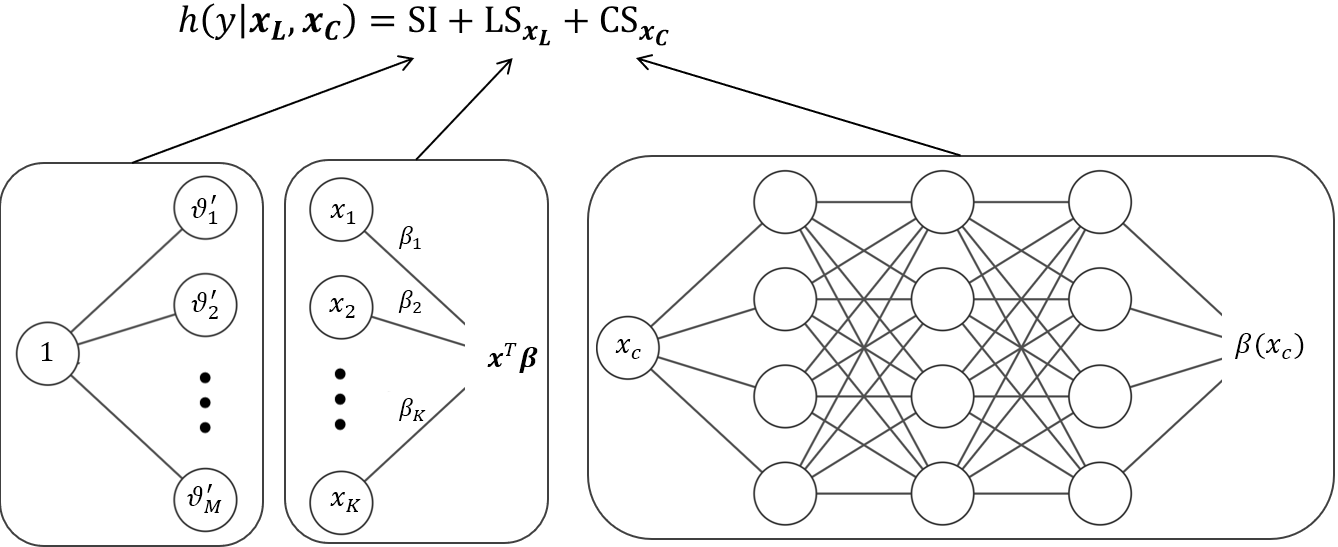
\includegraphics[width=0.9\textwidth]{img/deep_tram.png}
\caption{Modular deep transformation model. The transformation function $h(y \mid \mathbf{x})$ is constructed by the outputs of three neural networks.}
\label{fig:deep_tram}
\end{figure}

\textbf{Intercept } the shape of the transformation function at the baseline configuration $\mathbf{x}_L^\top \boldsymbol{\beta}_L = 0$ and $f_C(\mathbf{x}_C)=0$ is determined by the intercept $h_I(y)$. For a continuous outcome the intercept is represented by a smooth bernstein polynomial and in the discrete case by cut-points. In either case the parameters $\vartheta$ are obtained as output nodes of the neural network. A simple intercept (SI) is the case where the parameters $\vartheta$ do not depend on the any explanatory variables. The neural network thereby only takes a constant as input and directly outputs the parameters $\vartheta$. To make the intercept more flexible, the intercept can also depend on the explanatory variables. In this case the complex intercept (CI) models the intercept $\vartheta(x)$ by taking the predictors $x$ as input to a neural network with some hidden layers. This allows the intercept to change with the value of the predictors. Depending on the assumptions, predictors can be used in the complex intercept, or only a subset of them. A detailed explanation of the construction of the bernstein polynomial is given in appendix XXX.

\textbf{Linear shift } If the predictors should have a linear effect on the transformation function, it can be modelled by a linear shift (LS). For this part the neural network without hidden layers and without biases takes the linear predictors $pa(X_i)$ as input and generates a single output node with a linear activation function. This results in the linear combination $\mathbf{x}_L^\top \boldsymbol{\beta}_L$ and it induces a linear vertical shift of the transformation function. The weights $\boldsymbol{\beta}_L$ are the interpretable coefficients of the linear shift. For the logistic transformation model, they are interpreted as log-odds-ratios.
The interpretation is further described in the appendix XX.

\textbf{Complex shift } If the transformation function should be allowed to be shifted vertically in a non-linear manner, a complex shift (CS) can be applied. The predictor variables are inputed in a (deep) neural network with at least one hidden layer and a single output node with $f_C(X_C)$ is obtained. With a complex shift, also interactions between predictor variables can be captured.


\textbf{Level of complexity } One practical feature of these modular deep TRAMs is that one can specify, which predictors should have a linear or complex shift effect on the transformation function or that predictors are even allowed to deterimine the shape of the transformation function by a complex intercept. \citet{herzog2023} predicted the ordinal functional outcome three months after stroke by using semi-structured data that included tabular predictors and images. The two data modalities can be included in a single deep TRAM by modeling the part of the images with a CNN.

The estimated distribution function is invariant with respect to the choice of the inverse-link function $F_Z$ (scale of latent distribution) in an unconditional \citep{hothorn2018} or fully flexible (CI) setting. However, as soon as restrictions are placed on the influence of the predictors (LS, CS), this leads to assumptions about the scale of the dependency. Which latent distribution should be chosen depends on following factors: (i) the intended complexity of the model, (ii) the assumptions about the data generating process, (iii) the conventional, widely used, scale of interpretation for the specific problem. If the coefficients $\beta$ in the linear shift term should be interpreted as log odds ratios, then the standard logistic distribution is appropriate. For log hazard ratios it would be the minimum extreme value distribution. There exist plenty of other alternatives.

(The optimal scale could be found by comparing the likelihoods of the model under different latent distributions. )



\textbf{Parameter estimation } The parameters of the neural networks are learned by  minimizing the negative log-likelihood (NLL) of the conditional deep TRAM. The learning process is started with a random parameter configuration and the outputs of the neural networks are used to assemble the NLL of the transformation model. The NLL is then iteratively minimized by adjusting the parameters by the Adam optimizer \citep{kingma2015} until they eventually converge to the optimum state. Additionally, methods to prevent overfitting --- such as dropout, early stopping, or batch normalization --- can be applied. These techniques are particularly important in more complex networks to ensure that the model generalizes well to out-of-sample data. In the hidden layers, non-linear activation functions such as ReLU or sigmoid are applied.




\section{TRAM-DAGs}



In TRAM-DAGs these deep transformation models are applied in a causal setting. We assume a pre-specified DAG which defines the causal dependence. Then we estimate the distribution of each node by a transformation model that is conditional on its parents. Figrue \ref{fig:tram_dag} illustrates the basic idea of a TRAM-DAG where a DAG with 3 variables, without hidden confounder, is assumed to be known. The arrows in the DAG indicate the causal dependencies between the variables. The transformation models are constructed by a modular neural network. The assumed influence from the parent variables has to be specified as SI, LS or CS. In this example, $X_1$ is a continuous source node that acts as parent of $X_2$ and $X_3$. For a source node the transformation function only consists of a simple intercept (SI). $X_2$ is also continuous and its transformation function can be shifted additively (LS) by the value of $X_1$. $X_3$ is an ordinal variable with 4 levels and its transformation function depends on the values of $X_1$ (LS) and $X_2$ (CS). The cut-points $h(x_3 \mid x_1, x_2)$ represent the cumulative probabilities on the log-odds scale of the first 3 levels of $X_3$, where the probability of the last level $K=4$ is the complement of the previous levels $k_{1-3}$.

% include image /img/tram_dag.png
\begin{figure}[H]
\centering
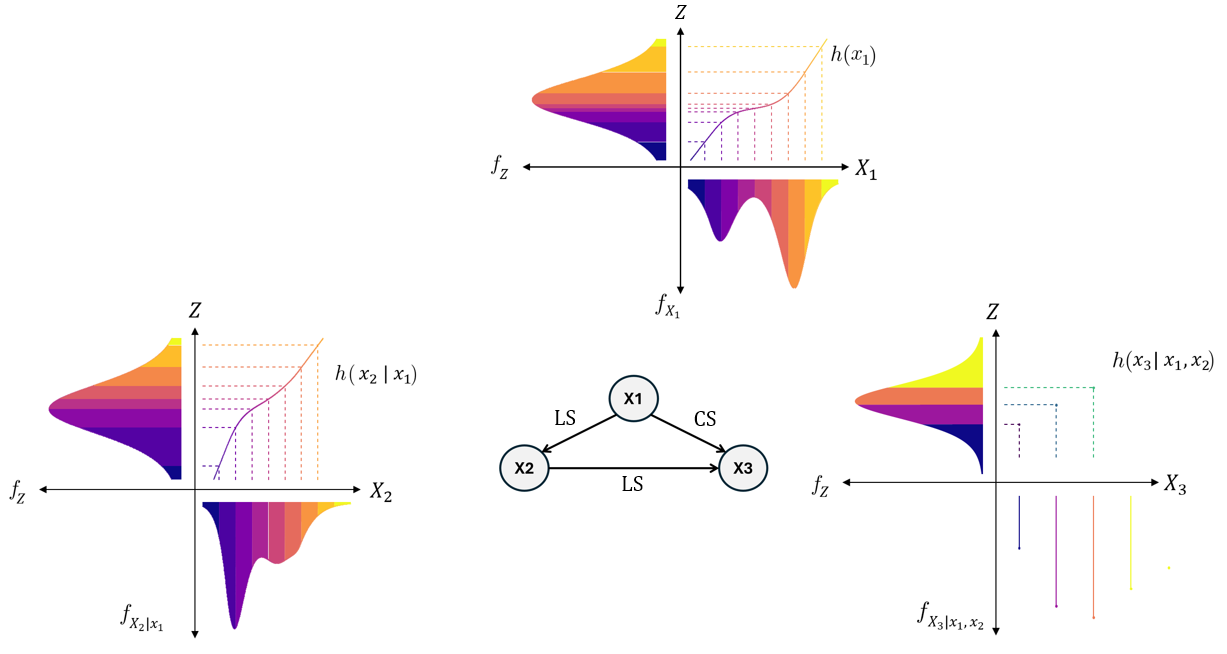
\includegraphics[width=0.9\textwidth]{img/tram_dag.png}
\caption{Example of a TRAM-DAG with three variables $X_1$, $X_2$ and $X_3$. The transformation functions are represented by the modular neural networks. The arrows indicate the causal dependencies between the variables.}
\label{fig:tram_dag}
\end{figure}

This DAG with the assumed dependencies can be described by an adjacency matrix \ref{eq:MA}, where the rows indicate the source and the columns the target of the effect: 


\begin{equation}
\mathbf{MA} =
\begin{bmatrix}
  0 & \text{LS} & \text{LS} \\
  0 & 0  & \text{CS} \\
  0 & 0  & 0
\end{bmatrix}
\label{eq:MA}
\end{equation}

To apply the framework of TRAM-DAGs on this example, we assume to have observational data that follows the structure of the adjacency matrix \ref{eq:MA}. In practice, the DAG is either defined by expert knowledge or by some sort of structure finding algorithm (XXX cite methods). Then we want to estimate the conditional distribution function of each variable by a deep TRAM so that we can sample from the distributions and make causal queries. The conditional distribution functions are given by


\[
\begin{aligned}
X_1 &\sim F_Z(h_I(x_1)) \\
X_2 &\sim F_Z(h_I(x_2) + \mathrm{LS}_{x_1}) \\
X_3 &\sim F_Z(h_I(x_3) + \mathrm{LS}_{x_1} + \mathrm{CS}_{x_2})
\end{aligned}
\]


\textbf{Construct Modular Neural network}

As discussed in the section \ref{sec:deep_trams}, the transformation functions are constructed by a modular neural network. The inputs are the variables in the system as well as the adjacency matrix \ref{eq:MA} which controls the information flow and assures that only valid connections according to the causal dependence are made. Discrete variables with few categories are dummy encoded, and continuous variables are scaled before feeding them in the neural network. The encoding and the effect of scaling on the interpretation of parameters is discussed in the appendix (ref XXX). The outputs are the three components for the transformation function (SI, LS, CS) for each variable. These components are assembled to the transformation functions. For the complex shift and complex intercept, the structure of the neural network (depth and width) has to be defined. 
Finally the loss is defined as the negative log likelihood, which the model aims to optimize to estimate the optimal parameterization. 


Describe interpretation quickly and refer to formal proof in the Appendix.
%  for interpretation see pearl book 2009 p. 366. the key is to say leaving all other variables "untouched" and not "constant". he also talks about the connection to the do-operator.

Finally, neural network works best if inputs are scaled. Proof that we can do that, it just changes the interpretation. For structure finding algorithms, this might be problematic, because increasing variance along the causal order would be destroyed. (why, how, interpretation change etc. check meeting notes 22.04.2025)

Fitting Betas Interpretable

The two parameters for our linear shift terms are plotted here. We can see that they converge quickly to the same values as we used in the DGP. We can interpret these parameters as log-odds ratios if changing the value of the parent by one unit.

Intercepts

Show the Discrete case with just cutpints (only K-1 parameters of outputs are used)
Show the continuous case where the outputs are transformed to monotonically increasing betas for the bernstein polynomial. Also describe Bernstein polynomial construction in detail with scaling and linear extrapolation.

Here I plotted the intercepts of the 3 transformation functions. They also resemble the DGP very nicely.


Linear and complex shifts

Here in the first two plots we can see the linear shifts. And in the right plot we have the complex shift of X2 on X3. The estimated shifts match quite well with the DGP.

Complex shift (Interaction example) to show what is also possible

Here I just want to make a short input from another example. So there the true model was that of a logistic regression with the binary outcome Y and 3 predictors. The binary treatment T and the two continuous predictors X1 and X2. There was also an interaction effect assumed between treatment and X1. So this basically means that the effect of X1 on the outcome is different for the two treatment groups.

And here we can show that our TRAM-DAG specified by a complex shift of T and X1 can also capture this interaction effect quite well.






\subsection{Sampling from TRAM-DAGs}

\textbf{Observational sampling} Once the TRAM-DAG is fitted on data, it can be used to sample from the observational or interventional distribution or to make counterfactual queries. 
The structural equations $X_i = f(Z_i, \text{pa}(X_i))$ are represented by the inverse of the conditional transformation functions $h^{-1}(Z_i \mid \text{pa}(X_i))$ because $Z_i = h(X_i \mid \text{pa}(X_i))$. The sampling process from the observational distribution for one iteration (one observation of all variables in the DAG) is described in the pseudocode \ref{alg:sampling} and illustrated in Figure~\ref{fig:sampling}. The process is repeated for the desired number of samples. 

\begin{algorithm}
\caption{Generate a samples from the TRAM-DAG}
\label{alg:sampling}
\begin{algorithmic}[1]
\State \textbf{Given:} A fitted TRAM-DAG with structural equations $X_i = f(Z_i, \text{pa}(X_i))$, where $Z_i = h(X_i \mid \text{pa}(X_i))$
\For{each node $X_i$ in topological order}
  \State Sample latent value $z_i \sim F_{Z_i}$ \Comment{e.g., \texttt{rlogis()} in R}
  \If{$X_i$ is continuous}
    \State Compute $x_i = h^{-1}(z_i \mid \text{pa}(x_i))$ by solving $h(x_i \mid \text{pa}(x_i)) - z_i = 0$
    \EndIf
  \If{$X_i$ is discrete}
    \State Determine $x_i$ such that $x_i = \min \left\{ x : z_i \le h(x \mid \text{pa}(x_i)) \right\}$
  \EndIf
\EndFor
\end{algorithmic}
\end{algorithm}


\begin{figure}[H]
\centering
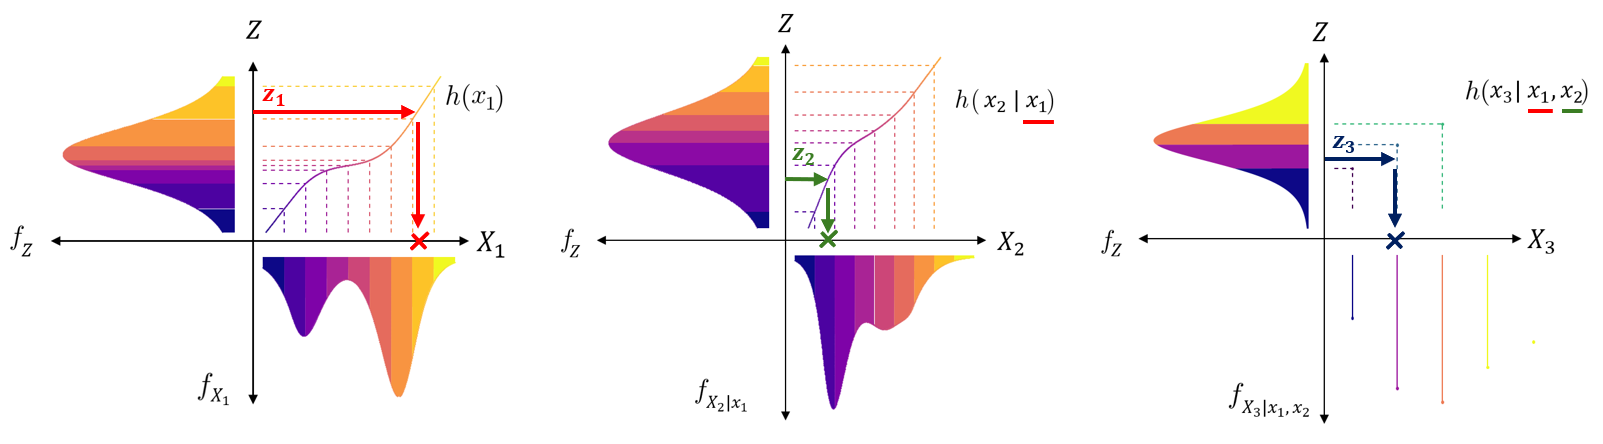
\includegraphics[width=0.9\textwidth]{img/sampling.png}
\caption{One sampling iteration for the three variables from the estimated transformation functions $h(x_i \mid \text{pa}(x_i))$. The latent values $z_i$ are sampled from the standard logistic distribution. The values $x_i$ are determined by applying the inverse of the transformation function for continuous variables or by finding the corresponding category for the ordinal variable.}
\label{fig:sampling}
\end{figure}


\textbf{Interventional sampling} To sample from the interventional distribution, we can apply the do-operator as described by \citet{pearl1995} (Pearl named it set instead of do). The do-operator fixes a variable at a certain value and sample from the distribution of the other variables while keeping the fixed variable constant. For example, if one wants to intervene on $X_2$ and set it to a specific value $\alpha$, $\textcolor{red}{\text{do}(x_2 = \alpha})$
and then sample from the interventional-distribution
\[
x_3 = \min \left\{ x : z_3 \le h(x \mid x_1, \textcolor{red}{x_2 = \alpha}) \right\}
\]

with the same process as for the observational sampling, with the only difference that the intervened variable $X_2$ stays constant.





\textbf{Counterfactual queries} In a counterfactual query one wants to know what the value of variable $X_i$ would have been if another variable $X_j$ had a different value than what was acutally observed. \citet{pearl_book2009} describes the three-step process to answer counterfacutal queries as follows: Given a causal model $M$ and observed evidence $e$ (which are the actually observed values of the variables $X_i$ of one sample) one wants to compute the probability of $Y=y$ under the hypothetical condition $X=x$.

Step 1 aims to explain the past (Z) by knowledge of the evidence e; 
Step 2 amends the past to the hypothetical condition $X=x$ 
Step 3 predicts the future (Y) based on our new understanding of the past and our newly established condition, $X =x$

Pearl named these three steps, (1) abduction,  (2) action and (3) prediction. The procedure is described in the pseudocode \ref{alg:counterfactual} and illustrated in Figure.

\begin{algorithm}
\caption{Answer a Single Counterfactual Query}
\label{alg:single_cf}
\begin{algorithmic}[1]
\State \textbf{Given:} A structural model $X_k = f(Z_k, \text{pa}(X_k))$, with inverse noise map $Z_k = h(X_k \mid \text{pa}(X_k))$
\State \textbf{Input:} Observed sample $x$, intervention $X_i := \alpha$, target variable $X_j$
\vspace{0.3em}
\State \textbf{Step 1: Abduction} Infer latent variable $Z_j = h(x_j \mid \text{pa}(x_j))$ using the observed values
\vspace{0.3em}
\State \textbf{Step 2: Action} Replace the value of $X_i$ with $\alpha$ in the set of parent variables
\vspace{0.3em}
\State \textbf{Step 3: Prediction} Compute the counterfactual value $x_j^{cf} = h_j^{-1}(Z_j \mid \text{pa}(x_j)^{cf})$
\vspace{0.3em}
\end{algorithmic}
\end{algorithm}



While the probability of Y under the hypothetical condition $X=x$ can be determined in any case, the actual counterfactual value of Y is only defined for a continuous outcome but not for discrete outcomes.

% see pearl book causality: 1.4.4 Counterfactuals in Functional Models (page 36)

(What pearl writes:  Likewise, in contrast with the potential-outcome framework, counterfactuals in the structural account are not treated as undefined primitives but rather as quantities to be derived from the more fundamental concepts of causal mechanisms and their structure. )


\textbf{ITE how it is applied in our model?}

% \citet{hoogland2021} gave guidance on how ITE estimation should be performed. A crucial aspect is the consideration is the model complexity and the susceptibility to overfitting. Also the decision whether a HGL or HTE model should be applied. (Especially include stuff from Practical Considerations part , quite good)
% RCTs only measure the average treatment effect. There will be patients who respond better or worse to the treatment because patient specific characteristcs. In personalized medicine however, the aim is to find the optimal treatment for a specific individual. Such a measure that can help in decision making is the ITE.

Rubins potential outcomes framework.


simulation studies
 "The setup was such that development and test sets were generated from the same data generating mechanism. In practice, there may be differences between these two settings that are not captured by the models, and the uncertainty that accompanies these unknowns may overshadow relatively small gains realized by more complex models."
 % https://pmc.ncbi.nlm.nih.gov/articles/PMC9291969/#sim9154-bib-0065
 
 "This could include the analysis of individual patient data from multiple randomized trials, or even the use of nonrandomized studies for the estimation of outcome risk under a control condition." this motivates the need for observational modeling.


Maybe it is the methods section. Here however, we give a couple hints.
Note that you can wisely use \rr{preamble}-chunks. Minimal, is likely:



Problems with ITE: (in an RCT setting)
- to estimate the ITE we must assume un-confoundedness. Does this also apply to itneractions (effect modifiers)? Check how this is handled in the literature.
- when there are treatment covariate interactions and these covariates are in the DGP but dropped from the dataset (so unobserved), then the ITE Estimation failed in the simulations. At least when there is only 1 strongly interacting variable and we drop this one. An example could be the psychological condition of a patient which might also affect how the treatment works, this is not a confounder but an effect modifier, and i would assume that this variable is rarely recorede or measured.

- Maybe a good conclusion: because this problematic with missing effect modifiers in RCT data can be a motivation to work with observational data where the dag is very detailed specified with all confounders and interactions, then a tram-dag can be applied. However, there we also have the problem, that important variables are probably also not known/measured...

- question still to answer: the estimated ITE on the train vs test set is equally bad (in terms of scatterplot and RMSE), so why does the ITE-cATE plot and the ITE Outcome plot looks like it discriminates good in the train set but not in the test set? Could the answer be, that the model is overfitting, hence tries to really model the observed outcomes and not the true probabilities, hence when an inportant variable is missing, it could still reasonably well predict the outcome (probability) but these are not the causal relationships anymore, so therefore the ITE estimation is bad on the train and the test set. But the ITE-cATE plot still looks good in the train set, because at least the observed outcomes could be predicted very well.??? still not sure if this is the case and how to proof.

- another point is the effect of the correlation of the variables. If the X's are strongly correlated, and one X with interaction effect is dropped, can the info then still be retreived from the other variables? --> check with simulations or theroretical proof.



\section{Experiments}

\subsection{TRAM-DAG simulation}

Show easy simulation with 3 variables and in the results the plots of the loss function, the coefficient learning, intercepts, shifts, and the sampling results. The sampling results should show that the sampled data matches the DGP very well. Also show the estimated parameters of the linear shifts and the intercepts. The complex shift can be shown by plotting the transformation function of X3 with respect to X2. also some queries for observational, interventional and counterfactual.

\subsection{TRAM-DAG real data}

maybe the Weather data case, or another if we find a practical observational data example.

\subsection{ITE simulations}

Show types of models that will be applied and dgp and when problems occure.

\subsection{ITE real data}

% describe the data of stroke trial https://pubmed.ncbi.nlm.nih.gov/9174558/
Results on IST trial wiht the interpretation in the discussion part.

show results of different models including tram dag.



\section{Software}

All code was done in R wiht packages xx ussed for yy.

\bigskip

\hrule
\begin{knitrout}
\definecolor{shadecolor}{rgb}{0.969, 0.969, 0.969}\color{fgcolor}\begin{kframe}
\begin{verbatim}
library(knitr)
opts_chunk$set(
    fig.path='figure/ch02_fig',
    self.contained=FALSE,
    cache=TRUE
)
\end{verbatim}
\end{kframe}
\end{knitrout}
\hrule

\bigskip

Defining figure options is very helpful:


\bigskip


\hrule
\begin{knitrout}
\definecolor{shadecolor}{rgb}{0.969, 0.969, 0.969}\color{fgcolor}\begin{kframe}
\begin{verbatim}
library(knitr)
opts_chunk$set(fig.path='figure/ch02_fig',
               echo=TRUE, message=FALSE,
               fig.width=8, fig.height=2.5,
               out.width='\\textwidth-3cm',
               message=FALSE, fig.align='center',
               background="gray98", tidy=FALSE, #tidy.opts=list(width.cutoff=60),
               cache=TRUE
)
options(width=74)
\end{verbatim}
\end{kframe}
\end{knitrout}
\hrule

\bigskip

This options are best placed in the main document at the beginning. Otherwise a \verb+cache=FALSE+ as knitr option is necessary to overrule a possible  \verb+cache=TRUE+ flag.

\bigskip

Notice how in Figure~\ref{f02:1} everything is properly scaled.

\begin{figure}
\begin{knitrout}
\definecolor{shadecolor}{rgb}{0.98, 0.98, 0.98}\color{fgcolor}

{\centering 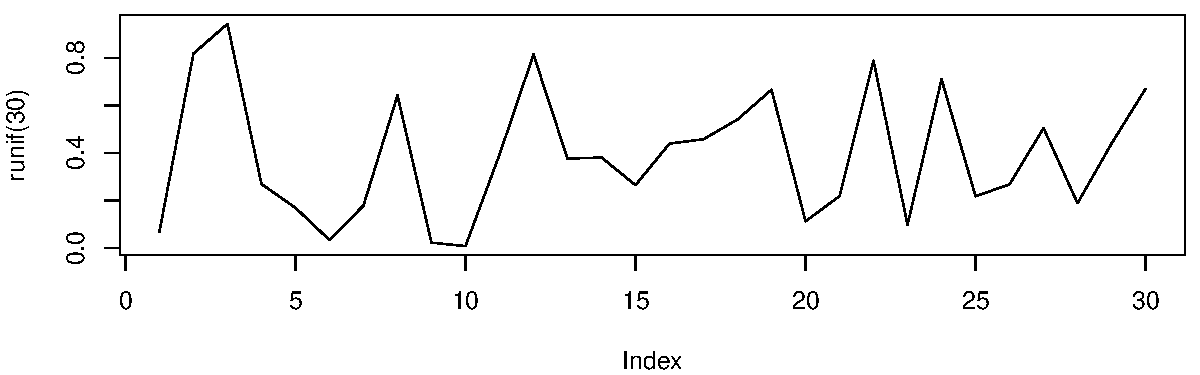
\includegraphics[width=\textwidth-3cm]{figure/ch02_figunnamed-chunk-3-1} 

}


\end{knitrout}
  \caption{Test figure to illustrate figure options used by knitr.}
  \label{f02:1}
\end{figure}


\section{Citations}

Recall the difference between \verb+\citet{}+ (e.g., \citet{Chu:Geor:99}), \verb+\citep{}+ (e.g., \citep{Chu:Geor:99}) and \verb+\citealp{}+ (e.g., \citealp{Chu:Geor:99}).
For simplicity, we include here all references in the file \verb+biblio.bib+ with the command \verb+\nocite{*}+.\nocite{*}

